\begin{figure}[]
	\begin{subfigure}{\linewidth}
		\caption{}
		\centering
		% include first image
		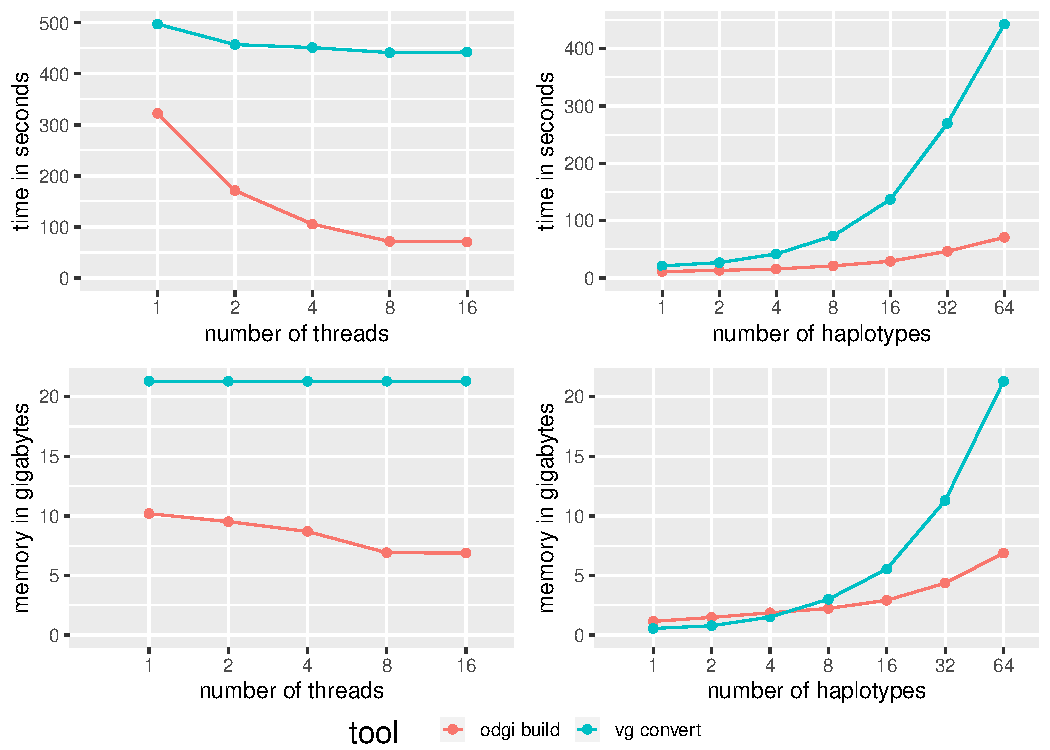
\includegraphics[width=1.0\linewidth, trim=0cm 1.25cm 0cm 0cm]{fig/performance/build_eval.pdf}
		\label{fig:eval-build}
	\end{subfigure}
	\begin{subfigure}{\linewidth}
	\caption{}
	\centering
	% include second image
	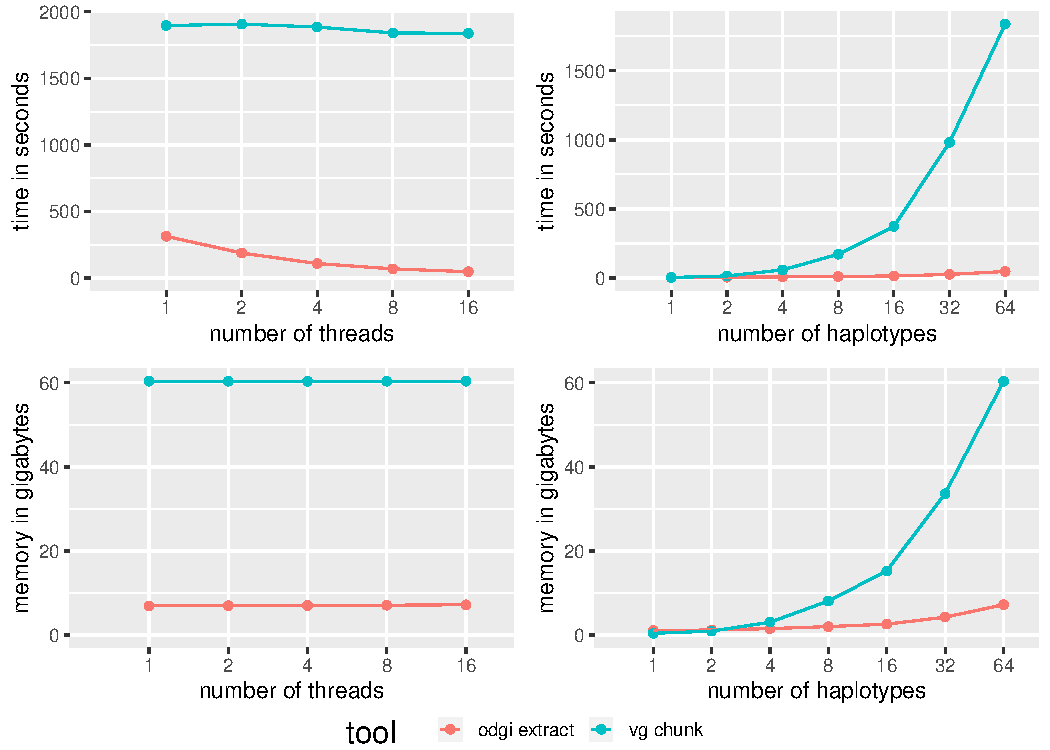
\includegraphics[width=\linewidth, trim=0cm 1.25cm 0cm 0cm]{fig/performance/extract_eval.pdf}
	\label{fig:eval-extract}
	\end{subfigure}
	\begin{subfigure}{1\linewidth}
		\caption{}
		\centering
		% include fourth image
		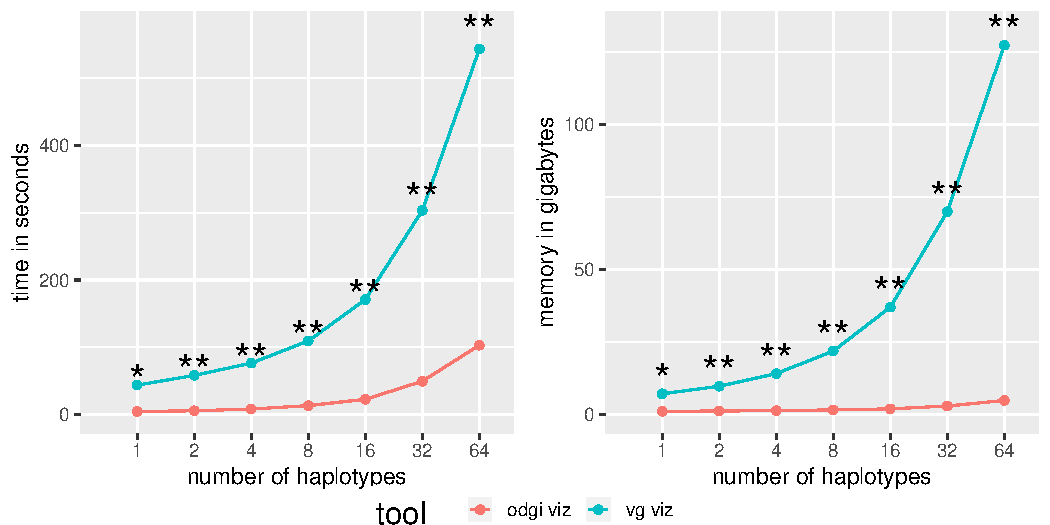
\includegraphics[width=\linewidth, trim=0cm 1.25cm 0cm 0cm]{fig/performance/viz_eval.pdf}
		\label{fig:eval-viz}
	\end{subfigure}
	\caption{\REVIEWED{Performance on a graph of human chromosome 6 from the HPRC. ODGI compares favorably to VG across all routine pangenomic tasks. Evaluations across threads were done using a 64 human haplotype graph. Evaluations across haplotypes were done using 16 threads. \textbf{(a)} Performance evaluation when translating a graph into the tools' respective native formats. \textbf{(b)} Performance evaluation when extracting the centromeric region from the HPRC graph. \textbf{(c)} Performance evaluation when visualizing a graph. Both tools were run with only one thread. \textit{vg viz}: \textbf{*}A 816MB SVG was produced which can't be opened by any program. \textbf{**}All produced SVGs only contain an XML header, nothing else.}}
	\label{fig:evaluation}
\end{figure}
